\subsection{Fravælgelse af gestik-par}
\label{TestresultaterSkiftDaarlig}
%
I følgende afsnit analyseres hvilke af de syv semaforiske gestik-par testpersonerne fravælger samt hvorfor testpersonerne netop fravælger disse gestik-par. På baggrund af analysen bør det være muligt at udpege hvilke semaforiske gestikker, der hvertfald ikke skal knyttes til at skifte musiknummer. Analysen bygger på testpersonerne respons til spørgsmålet: \textit{Hvilken gestik kan du mindst lide? og hvorfor?}, hvor testpersonernes samlede data er vedlagt i ELEKTRONISK BILAG.
%
\begin{figure}[H]
	\centering
	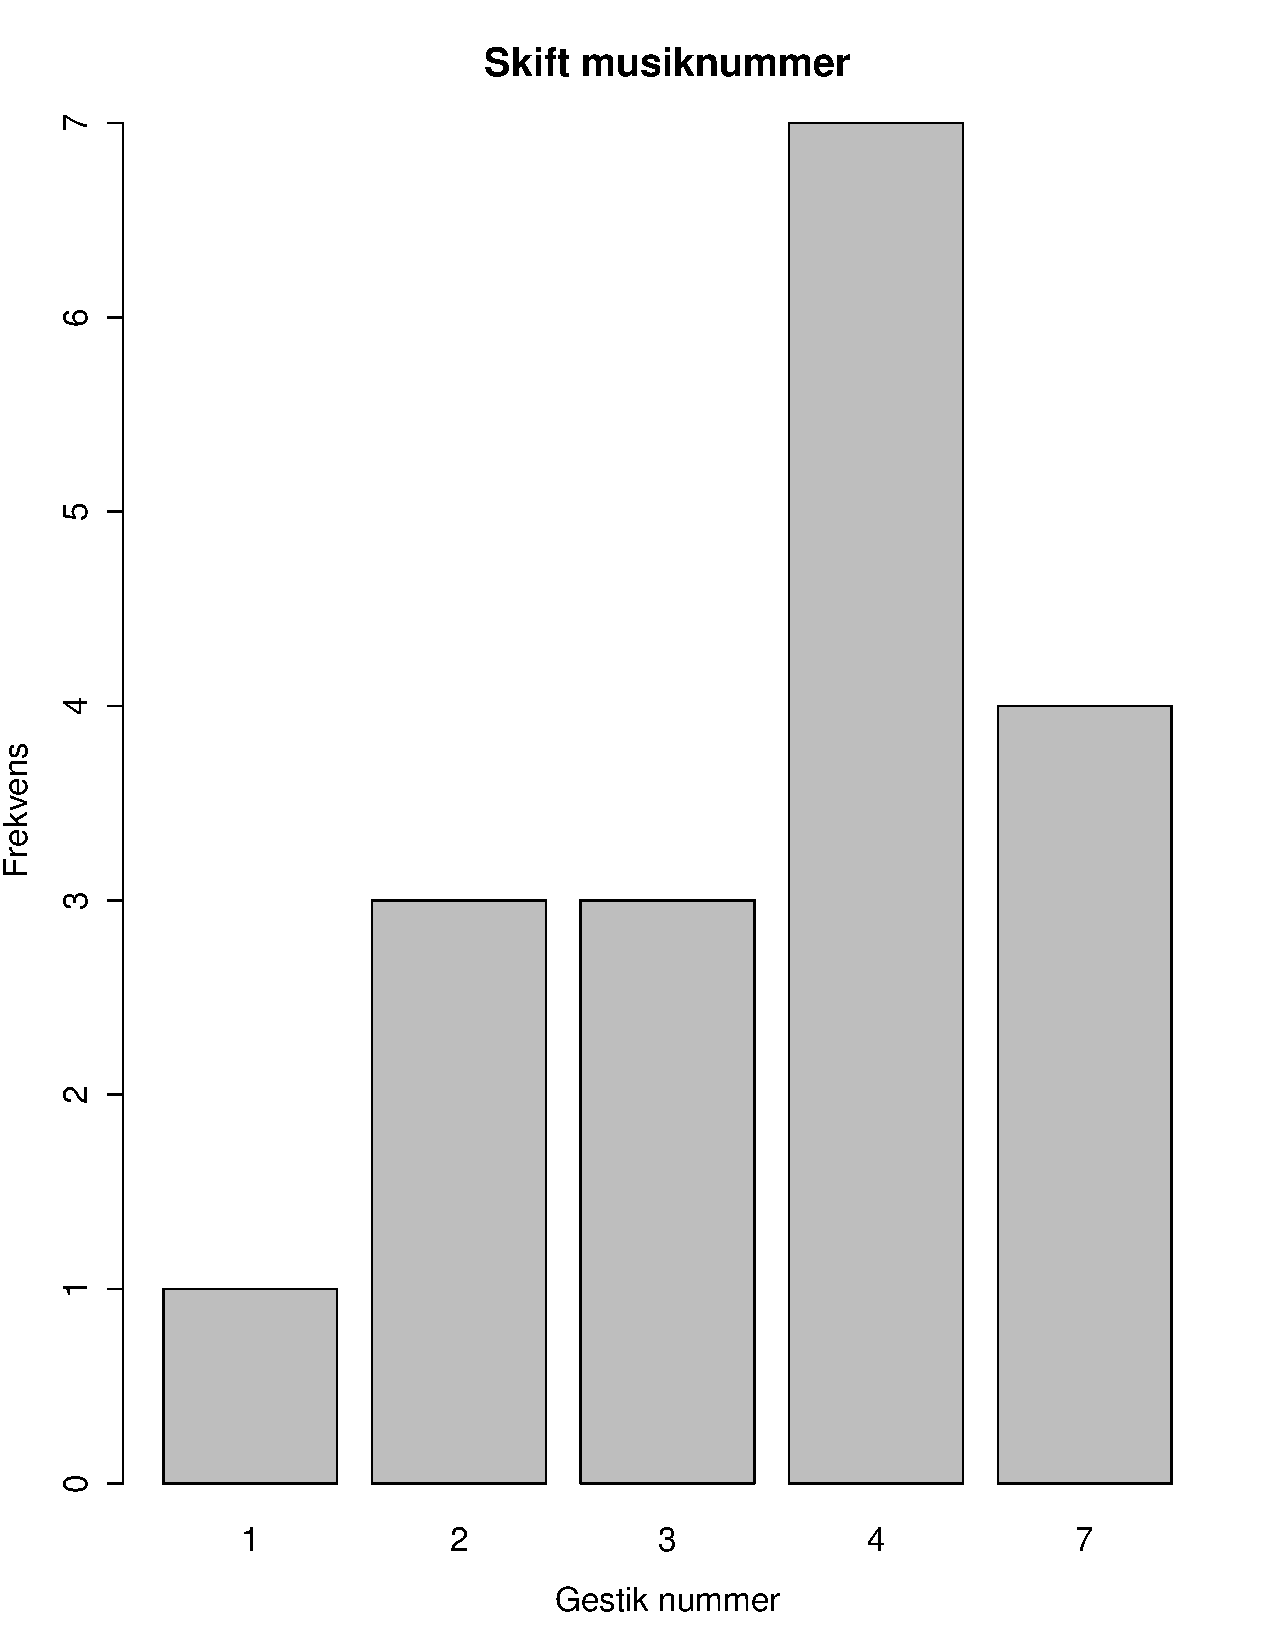
\includegraphics[resolution=300,width=0.5\textwidth]{Test1/DatabehandlingGrafer/DaarligstGestikSkift.pdf}
	\caption{Barplot over hvilke gestik-par testpersonerne fravælger i forbindelse med at skifte musiknummer frem og tilbage. Søjlerne bygger på testpersonernes respons, hvorfor det kun er de fravalgte gestik-par, der udgør plottet.}
	\label{fig:DaarligstGestikSkift}
\end{figure}
\noindent
%
På \autoref{fig:DaarligstGestikSkift} fremgår det hvilke gestik-par de 18 testpersoner fravælger i forbindelse med at skifte musiknummer. Det fremgår tydeligt at gestik-par 4 er det par, som flest testpersoner fravælger i forhold til de resterende par på \autoref{fig:DaarligstGestikSkift}. Årsagen til at testperson 14 har valgt gestik-par 1, som værende den testpersonen mindst kan lide, begrundes med at testpersonen forestiller sig, at det er en bevægelse testpersonen vil komme til at gøre gentagende gange foran sit anlæg eller under en samtale. Testperson 1, testperson 5 og testperson 16 har alle valgt gestik-par 2, som værende den de mindst kan lide, fordi gestikken er modsat af, hvad de forventer er frem og tilbage. At gestik-par 3 fravælges begrunder testperson 3, testperson 11 og testperson 13 med at hvis der skulle peges i en retning så skulle det være med pegefingeren og ikke tommelfingeren, det er en akavet bevægelse og fordi gestikken er statisk. I den forbindelse kommenterer testperson 5 at vedkommende heller ikke bryder sig om hverken gestik-par 3 eller gestik-par 7, netop fordi de er statiske.

Der er forskellige årsager til at syv testpersoner fravælger gestik-par 4. Testperson 4 og testperson 6 fravælger gestikken fordi den er mærkelig, hvor testperson 4 forbinder det med at skulle tage telefonen. Testperson 8 forstår ikke hvorfor det er lige præcis er det håndtegn der skal bruges. Testperson 10 oplever ikke at gestikken bringer noget nyt men snarre er en besværlig version af gestik-par 5. I forhold til håndtegnet i gestik-par 4, så kommenterer testperson 12 at det er unaturligt at gøre noget med lillefingere, testperson 7 kommenterer dels at det er en stor armbevægelse og dels at det er et sjovt håndtegn, som vil blive glemt, hvis det ikke bliver brugt. I tillæg kommenterer testperson 18 ligeledes at det er en unaturlig gestik, som vil blive glemt dog pointerer testpersonen at det er en effektiv gestik i og med at den ikke vil blive lavet ved en fejl. 

Årsagen til at gestik-par 7 fravælges skyldes ifølge testperson 2, testperson 9 og testperson 17, dels at den virkede mærkelig, dels at den ikke blev opfattet og dels at den minder lidt om en pistol. Ligesom gestik-par 3 blandt andet blev fravalgt fordi den er statisk, så fravælger testperson 15 af samme årsag gestik-par 7 og fordi det er et enkelt tegn.\blankline
%
For at afgøre hvilke af de syv gestik-par, der skal fravælges er det nødvendigt at sammenholde hvilke gestikker testpersonerne fravælger med de gestikker, som indgår i testpersonernes top tre rangering. Der opstilles derfor en tabel over de fem fravalgte gestik-par og hvordan de indgår i testpersonernes rangering.    
%
\begin{table}[H]
	\centering
	\begin{tabular}{ | p{1.5cm} | p{2.1cm} | p{2.1cm} | p{2.1cm} | p{2.1cm} | p{2.1cm} |}
	\hline
		 & Gestik-par 1 & Gestik-par 2 & Gestik-par 3 & Gestik-par 4 & Gestik-par 7 \\ \hline
		1. Plads & 10 & 3 & 1 & 0 & 0\\ \hline
		2. Plads & 2 & 3 & 3 & 0 & 1\\ \hline
		3. Plads & 0 & 0 & 7 & 5 & 2\\ \hline
	\end{tabular}
	\caption{Oversigt over hvor ofte og hvor de fem fravalgte gestikker indgår i testpersonernes top tre rangering.}
	\label{tab:FravalgteTopTreSkift}
\end{table}
\noindent
%
På baggrund af \autoref{tab:FravalgteTopTreSkift} sammenholdt med \autoref{fig:DaarligstGestikSkift}, tyder det på at gestik-par 4 og gestik-par 7 kan ekskluderes fra fremtidige undersøgelser. Det skyldes at selvom gestik-par 4 indgår fem gange i testpersonernes top tre, så fravælges parret af syv testpersoner. Derudover tyder det på, at de fem testpersoner, som har inkluderet gestik-par 4 i deres top tre, har gjort det på baggrund af bevægelsen snarre end kombinationen af både håndtegnet og bevægelsen. Gestik-par 7 ekskluderes da parret kun indgår tre gange i top tre og da den derudover fravælges af fire testpersoner. 

De tre testpersoner, som fravælger gestik-par 2, gør det formentligt fordi de har en mental model af, at hvis der swipes fra højre mod venstre så afspilles det næste musiknummer i playlisten, modsat hvis der swipes fra venstre mod højre så afspilles det forrige musiknummer. Hvorimod de tre testpersoner, der har inkluderet gestik-par 2, som deres første valg, formentligt har den modsatte mentale model af hvilken swipe bevægelse der skal udføres for at skifte til det næste musiknummer. For at det kan afgøres hvorvidt gestik-par 2 skal ekskluderes eller ej, så er det nødvendigt at undersøge nærmere hvilke gestik-par de seks testpersoner, som har inkluderet gestik-par 2 i deres top tre, ellers har inkluderet. 
%
\begin{table}[H]
	\centering
	\begin{tabular}{ | p{3cm} | p{3cm} | p{3cm} | p{3cm} |}
	\hline
		 & 1. Plads & 2. Plads & 3. Plads \\ \hline
		Testperson 4 & Gestik-par 2 & Gestik-par 5 & Gestik-par 3 \\ \hline
		Testperson 17 & Gestik-par 2 & Gestik-par 3 & Gestik-par 4 \\ \hline
		Testperson 18 & Gestik-par 2 & Gestik-par 1 & Gestik-par 3 \\ \hline
		Testperson 8 & Gestik-par 3 & Gestik-par 2 & Gestik-par 7 \\ \hline
		Testperson 12 & Gestik-par 1 & Gestik-par 2 & Gestik-par 5\\ \hline
		Testperson 15 & Gestik-par 1 & Gestik-par 2 & Gestik-par 5 \\ \hline
	\end{tabular}
	\caption{Oversigt over de seks testpersoner, som enten har tildelt gestik-par 2 en første eller en anden plads i top tre, samt hvilke gestik-par de ellers har inkluderet.}
	\label{tab:GestikPar2ITopTre}
\end{table}
\noindent
%
Sammenholdes testperson 4's top tre rangering med testpersonens udsagn og bevægelser i videooptagelserne, så tyder det på at denne testperson har en mental model af at hvis der swipes fra højre mod venstre så afspilles det forrige musiknummer kontra et swipe fra venstre mod højre, som vil afspille det næste musiknummer. Testpersonen kommenterer ydermere at gestik-par 5 også vil fungere såfremt retning var omvendt, svarende til hvad der sker i gestik-par 2. Testperson 17, som også har rangeret gestik-par 2 som det bedste, udfører også de korrekte bevægelser i forhold til testpersonens egne kommenterer, dog opstår der en smule usikkerhed, når testpersonen afslutningsvist skal gengive sine fortrukne gestikker. Efter en diskusion frem og tilbage med testlederen konkluderer testperson 17 dog at det stadig er gestik-par 2, der er bedst. Selvom testperson 18 virker sikker i sit valg om, at det er gestik-par 2, der er det bedste gestik-par, så gengiver testpersonen rent faktisk bevægelserne fra gestik-par 1, dog med venstre hånd. Når testpersonen i tillæg forklarer hvad swipe bevægelserne gør i forhold til at skifte til det forrige eller det næste musiknummer, relaterer det sig ligeledes til gestik-par 1. Det er derfor ikke til at vide hvorfor testpersonen har rangeret gestik-par 2 højere end gestik-par 1. Det tyder derfor på at den eneste testperson, der med sikkerhed vil vælge swipe bevægelserne i gestik-par 2, er testperson 4. 

Rettes fokus mod de tre testpersoner, som har rangeret gestik-par 2 på en anden plads, så tyder det på at de to testpersoner, som har gestik-par 1 på en første plads, hovedsageligt har inkluderet gestik-par 2 på grund af bevægelsen. Dog kommenterer testperson 15, at gestik-par 2 er modsat af hvad testpersonen finder logisk, i forhold til at skifte musiknummer.  Derudover pointere testperson 12 at det var svært at adskille gestik-par 1 fra gestik-par 2. Testperson 8 har derimod rangeret gestik-par to mellem de to statiske gestik-par og når testpersonen gengiver bevægelserne for gestik-par 2 så stemmer det både overens med testpersons udsagn samt hvordan gestik-parret er designet. Det tyder derfor på at testpersonen rent faktisk har valgt gestik-par 2 fordi det stemmer overens med testpersonens mentale model.\blankline 
%
Ud af de seks testpersoner er det kun testperson 4 og testperson 8, der rent faktisk giver entydigt udtryk for at deres mentale model af gestik-par 2 stemmeroverens både med deres bevægelser og deres udsagn. Derudover er der i Bang $\&$ Olufsen's produkter desuden truffet en design beslutning om, at en swipe bevægelse fra højre mod venstre resulterer i at det er det næste musiknummer, der afspilles. På baggrund af den foregående analyse og da det ikke ønskes at gå i mod Bang $\&$ Olufsen's designvalg, vurderes det derfor at der er tilstrækkeligt belæg for at ekskludere gestik-par 2. 

På baggrund af foregående analyse forefindes der ikke et tilstrækkeligt belæg for hverken at ekskludere gestik-par 1 eller gestik-par 3. 

